% [5~r\textsuperscript{o}]
% \vspace{1em}%
\pstart%
% \noindent%
\edtext{}{\lemma{}\Afootnote{\textit{Am oberen Rand von Bl. 5~r\textsuperscript{o}:} Observationum Anatomicarum ex Mso. Cartesii\protect\index{Namensregister}{\textso{Descartes}, Ren\'{e} (1596-1650)} (II)}}
% \pend%
% \pstart%
Secta posthac gula in directum reperi adhuc herbarum frustula intus indigesta, unde mihi innotuit hunc vitulum fuisse grandiorem natu quam mihi erat relatum, jamque herbas comedisse quae ibi in palearibus haerebant.%
\edtext{}{\lemma{}\Afootnote{\textit{Am Rand:} Imo erat maxime juvenis (+ adscriptum in margine +).\vspace{-4mm}}}
\pend%
\pstart%
Notavi etiam in aspera arteria, duos inferiores ramos ex eodem annulo infimo et latiori emergere; 3\textsuperscript{tium} vero dextrum 7\textsuperscript{em} altius et in reliqua denique arteria quamvis totam non haberem, 40 tamen annulos numeravi, quot fuerint amplius ignoro.
\pend%
\pstart%
Dixi quidem \edtext{supra}{\lemma{supra}\Cfootnote{Siehe oben, S.~\pageref{jamcirca}.}}
quo pacto venulae et arteriolae in cordis superficie apparerent. Fibrae autem ex quibus ipsa cordis caro constat in alias partes flectuntur, nempe vel omnes perpendiculariter vel certe potius a dextra ad pectus, nec sane ventriculorum distinctio in illis est cujusdam momenti, sed recte consideranti videtur tota cordis caro ab impulsu cavae facta esse quae mittebat sanguinem versus mucronem, et inde major ejus pars in partem sinistram flectebatur. Qui vero spiritus erant subtiliores, magis versus medium cordis sive ipsam motus originem reflectebantur;
in aorta qui crassiores supra erant in venam arteriosam, qui vero subtilissimi per cordis carnem evadebant reflectebantur deorsum in exiguum istud foramen quod
notavi % LH IV 1,4B Bl. 4~v\textsuperscript{o}, Z. 63, hier 
esse infra cavam ibique sequebantur vestigia primae venulae (quo solo in loco vasa cordis
\edtext{[cutanea]}{\lemma{cutacea}\Bfootnote{\textit{L \"{a}ndert Hrsg.}}} et ejus fibrae eandem viam
\pend
\newpage
\pstart\noindent servant) ac deinde in spatio intra pericardium contento dispergebantur; ibique condensati ipsum cor vel alebant, vel certe conservabant. (In via autem ista primae venulae carnis fibrae utrinque latiores in basi cordis versus mucronem in illam confluebant pari modo utrinque non tam accurate, sed sinistrae magis versus mucronem in dextrum flectebantur[)]. Jam sumendo sinum duos ramos aortae et venam arteriosam, videbatur facere unicum vas ex anteriore cordis basi egrediens, contra auriculae utrinque cum carne intermedia partem instar valli cingebant per quam partem tum cava, tum arteria venosa et cavae propago sinistra in cor penetrabant: haec cavae propago est haud dubie coronaria dicta, et ubi habet ortum a cava disseminat omnes venulas quas \edtext{supra}{\lemma{supra}\Cfootnote{Siehe oben, S.~\pageref{jamcirca}.}} notavi esse in superficie cordis, quae ideo vergunt in alias partes quam fibrae \edtext{cordis[;] basi}{\lemma{}\Bfootnote{fibrae cordis[;] \textbar\ quae \textit{streicht Hrsg.} \textbar\ basi \textit{ L}}} cordis crescente magis \edtext{quam mucro}{\lemma{quam}\Bfootnote{\textit{(1)}\ juncta \textit{(2)}\ mucro \textit{L}}} harum fibrarum extrema locis quibus adhaerebant manserunt affixa.
\pend%
\pstart%
\begin{wrapfigure}[11]{l}{0.4\textwidth}
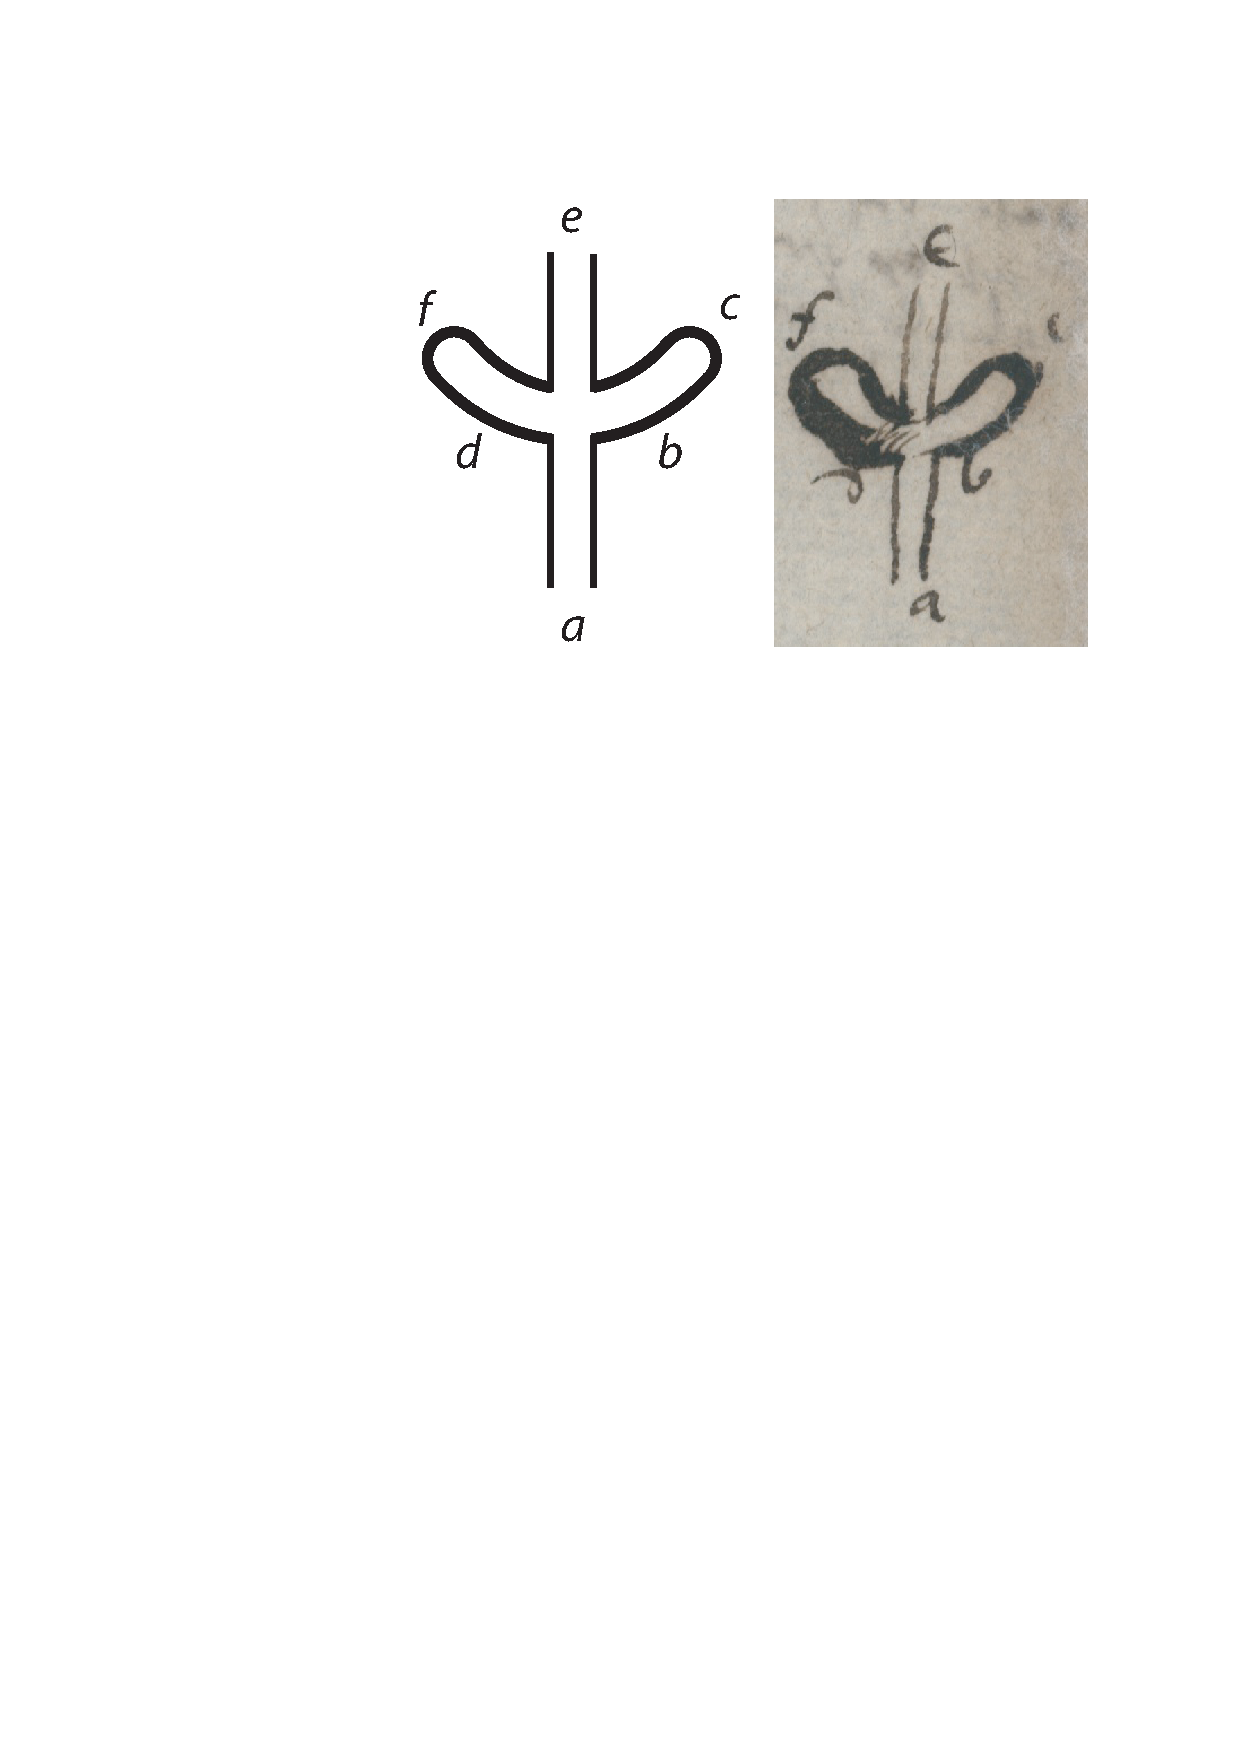
\includegraphics[trim = 0mm -3mm -5mm 0mm, clip, width=0.4\textwidth]{images/lh0040104b_005r.pdf}\\
\centering [\textit{Fig. 6}]
\end{wrapfigure}%
Apertis postea vena cava in directum et duabus auriculis et coronaria, vidi istam coronariam ab origine mucronem versus descendentem ibi paulatim ex corde se subtrahere, cum interim meatus essent transversi in fibris cordis per quos in cor rursus penetrabat, quicquid per illam egredi conabatur; eodem modo ramus ejus praecipuus per medium parietem transiens excipiebatur a quatuor aut quinque exiguis foraminibus in basi cordis si quid crassius per illam effluebat ex quibus unum directe respondebat illi supra notato infra cavae ingressum in cordis cute. Vidi quoque distincte partem cavae inclusam in pericardio plane ejusdem fuisse substantiae atque auriculas cavamque ab initio sursum ascendentem ocurrente illi obstaculo stagnasse in pectore,
ibique in molem $fbc$ ex duabus auriculis et carne media concrevisse, postea vero exitum sibi fecisse, tum sursum versus pectus per $e,$ tum versus spinam in pulmones per
\edtext{[$a$]}{\lemma{$d$ }\Bfootnote{\textit{L \"{a}ndert Hrsg.}}}
arteriam venosam; ac praeterea in medio istius molis carneae cor formasse, tandemque in illud et per $b$ et per valvulam inter $b$ et $d$ suos ventriculos excavasse; valvula enim ista adhaerebat moli carneae in parte $i$ per quasdam fibras, ita ut pateret sanguinem quidem semper decidisse per illam ex cava in sinistrum ventriculum, nunquam vero quicquam ex sinistro ventriculo in
\edtext{[dextrum]}{\lemma{dextram}\Bfootnote{\textit{L \"{a}ndert Hrsg.}}}
vel cavam, sed quod ex sini-
\pend
\newpage
\pstart\noindent stro ventriculo redundabat in pulmones, ibat per arteriam venosam, ex qua rursus in cor regurgitabat, ex qua regurgitatione formata est valvula $bi.$
\pend%
\pstart%
Erat os dextrum cavae in cor triangulare quodammodo unde 3 ibi valvulae, os vero tum cavae tum arteriae venosae in sinistrum quasi ovale, unde tantum duae, idque ex conjunctione sinuum necessario sequebantur.
\pend%
\pstart%
Apertis postea aorta et vena arteriosa praeter vulgaria omnia animadverti tres venae valvulas vix totas posse aperiri claudi autem quam maxime carne scilicet intra ipsas protuberante, item valvulam aortae quae pectus respiciebat, eodem modo aperiri vix posse propter eandem rationem, sed alias duas e contra vix claudi posse, quod juvat ad cognoscendum, cur major vis in sinistro latere confluxerit. Denique ibi observavi nervum (sexti paris ut puto) in cor absumi inter aortam et venam versus anteriorem partem, jungebantur autem aorta et vena in communi valvularum interstitio indissolubiliter. Excussi deinde venas et arterias cutaneas venae erant 1\textsuperscript{a} ex 4 venulis perpendicularis ad mucronem ex cava et secunda ex propagine cavae cutanea, et alia inter utramque in basi cujus originem, non vidi apparentem, nec item aliarum quae deorsum ex ea descendebant quamvis caeterae magis sanguineae apparerent, puta propter situm. 3\textsuperscript{tia} et 4\textsuperscript{ta} ex supra nominatis simul veniebant a ramo ex aorta in medio valvulae posterioris exeunte. Ramus autem ex medio valvulae anterioris (de quibus supra) exibat quidem in cutem ex medio cordis versus finem auriculae dextrae, sed majori ex parte in ipsum cor rursus absumebatur: caeterum venae istae cutaneae et arteriae non poterant ab invicem visu distingui nec alio modo nisi ratione originum, earumque tunicae erant versus extrema tenuissimae et facile a cordis carne separabantur et perforabantur in extremis.
[5~v\textsuperscript{o}]
\pend
%\count\Bfootins=1500
%\count\Cfootins=1500
%\count\Afootins=1500